\chapter{静磁学、时变场}
\label{chap:magnetostatics}
本章主要介绍静磁学(magnetostatics)的内容,与前几章介绍的静电学在多处均有呼应。%当然,本文为节省篇幅省略了一些科学史的介绍及磁学的发展研究历程,感兴趣的读者可以自行查找相关资料了解。同时,对于一些过于基础性的概念也仅仅只做大致的描述。
类似于静电学,我们建立了静磁学的基本方程组,通过几个边值问题阐述了静磁学问题的处理方法。%(如均匀带电圆环在全空间产生的磁场……)。
%,……
%第三节介绍似稳场(quasi-static field)理论,……

第二节介绍Faraday定律,将静电学和静磁学中的恒稳态问题变为与时间有关的时变场(time-varying field)问题。

\section{磁感应强度、电流密度}
\label{sec:introduction to magnetostatics}

%值得注意的是,
磁场(magnetic field)的基本规律最早并不是直接根据人类对磁性材料的接触中得出的,原因在于静磁学和静电学存在一个根本上的差别:人们没有发现自由磁荷(free magnetic charge)的存在。在磁学中,基本单元是磁偶极子\footnote{就是高中物理里的小磁针模型。}(magnetic dipole)。磁场的磁感应强度\footnote{也称磁通密度(magnetic-flux density)}(magnetic induction) $\bm B$其方向被定义为处在该磁场中的磁偶极矩$\bm\mu$的方向,其大小可以由磁偶极矩$\bm\mu$所受力矩$\bm N$来衡量:
\begin{equation}
    \bm N=\bm\mu\times\bm B.
\end{equation}
另外通过Ørsted等人的实验,我们可以知道磁场是由电流(current)产生的。电流相当于运动电荷,用电流密度(current density)矢量$\bm J$描述:
\begin{equation}
    \bm J:=\rho\bm v,
\end{equation}
其大小为单位时间流过单位面积的电荷量,其方向为电荷运动的方向。
\paragraph{连续性方程}
由于电荷守恒(conservation of charge),空间中固定一点的电荷量不会有源项,因此
\begin{equation}
    \label{eqn:continuity}
    \pv\rho t+\div\bm J=0,
\end{equation}
上式称为连续性方程(continuity equation)。上式也可通过另一种方式推导:考虑空间一体积微元$V$,其内电荷量不随时间改变:
\begin{equation*}
    \label{eqn:d(rhoV)/dt=0}
    \dv{(\rho V)}t=\dv\rho tV+\rho\dv Vt=0,\tag{$\ast$}
\end{equation*}
由于$\rho=\rho(x,y,z,t)$是时空的函数,其全微分为
\[
    \d\rho=\pv\rho t\d t+\pv\rho x\d x+\pv\rho y\d y+\pv\rho z\d z,
\]
两端除以$\d t$,得到其迁移导数(convective derivative)为
\[
    \dv\rho t=\pv\rho t+\pv\rho xv_x+\pv\rho yv_y+\pv\rho zv_z=\pv\rho t+\bm v\cdot\nabla\rho;
\]
而体积元的变化率
\[
    \dv Vt=\oint_{\p V}\bm v\cdot\d\bm a=\int_V\div\bm v\d V=V\div\bm v.
\]
因此\eqref{eqn:d(rhoV)/dt=0}变为
\[
    \dv\rho t+\rho\div\bm v=\pv\rho t+\bm v\cdot\nabla\rho+\rho\div\bm v=\pv\rho t+\div(\rho\bm v)=0,
\]
上式即\eqref{eqn:continuity}。
\paragraph{稳恒电流}
稳恒(steady-state)磁现象满足空间各处的$\rho$不变,于是%对于静磁学,
\begin{equation}
    \div\bm J=0.
\end{equation}
%我们从电流与磁感应强度之间的关系出发,建立静磁学基本定律。

\section{Biot-Savart定律}
\label{sec:Biot-Savart law}

%尽管磁现象的发现有很悠久的历史,但直到建立了电流和磁场之间的联系,磁现象才得到定量描述。
为了描述电流在激发磁场时的作用,我们引入电流元(current element)的概念:$\d\bm\ell$是通电流$I$的导线的长度元,指向电流方向,则电流元为$I\d\bm\ell$。
\begin{theorem}{Biot-Savart定律}{Biot and Savart Law}
    原点处电流元$I\d\bm\ell$在$\bm x$处激发的磁感应强度元$\d\bm B$为
    \begin{equation}
        \label{eqn:B-S law}
        \d\bm B=k\frac{I\d\bm\ell\times\bm x}{|\bm x|^3},\quad k=\frac{\mu_0}{4\pi},
    \end{equation}
    真空磁导率$\mu_0\simeq 4\pi\times{10^{-7}}\,\si{N/A^2}.$
\end{theorem}
尽管式\eqref{eqn:B-S law}与点电荷电场强度\eqref{eqn:E of q}有相似的形式,但%电流元$I\d\bm\ell$并不能视为点电荷$q$的磁场对应,
%只有把电流元看做对连续集合(电流回路)求和中的一个元素时才有意义,
式\eqref{eqn:B-S law}只有在积分中才有意义,
因为电流元本身并不满足连续性方程\eqref{eqn:continuity}。
\footnote{一种摆脱这个困难的办法是将电流元$I\d\bm\ell$换成运动电荷$q\bm v$
\[
    \bm B=k\frac{q\bm v\times\bm x}{|\bm x|^3}.
\]
但这个表达式与时间相关,并且只有当电荷速度$v\ll c$且加速度可忽略不计时才成立。
而式\eqref{eqn:B-S law}则是精确的:
对于一个电荷单元趋于0且电荷数目趋于无穷大的稳恒电流系统,相对论电磁场理论(包括加速度效应)将给出一个静磁场,并且形式上等于对式\eqref{eqn:B-S law}遍历电流积分所得的场。所以我们采用\eqref{eqn:B-S law}。}
\begin{example}{无限长直导线的磁场}{B of straight line}
    $z$轴上的长直导线电流方向为$+z$,距离其$\rho$处的磁感应强度大小为
    \[
        B_\phi(\rho)=\frac{\mu_0}{4\pi}\int\iti\frac{I\rho\d z}{(z^2+\rho^2)^{3/2}}=\frac{\mu_0}{2\pi}\frac I\rho.
    \]
    方向服从右手定则,即$\uvec\phi$方向。
\end{example}
电流元$I\d\bm\ell$在磁感应强度$\bm B$中所受的力
\[
    \d\bm F=I\d\bm\ell\times\bm B.
\]
换成电荷得到磁场的Lorentz力
\begin{equation}
    \bm F=q\bm v\times\bm B.
\end{equation}
\begin{example}{闭合回路之间的力}{F of 2 closed lines}
    由闭合电流回路2产生的磁场$\bm B$对闭合电流回路1的总力:
    \[
        \bm F_{12}=\frac{\mu_0}{4\pi}I_1I_2\oint\oint\frac{\d\bm\ell_1\times(\d\bm\ell_2\times\bm x_{12})}{|\bm x_{12}|^3};
    \]
    利用\eqref{eqn:bac-cab}将双叉乘化为更对称的形式:
    %\bm A\times(\bm B\times\bm C)=\bm B(\bm A\cdot\bm C)-\bm C(\bm A\cdot\bm B)
    \[
        \bm F_{12}=\frac{\mu_0}{4\pi}I_1I_2\biggfkh{\oint\cancel{\oint\frac{\bm x_{12}\cdot\d\bm\ell_1}{|\bm x_{12}|^3}}\d\bm\ell_2-\oint\oint\frac{\bm x_{12}}{|\bm x_{12}|^3}(\d\bm\ell_1\cdot\d\bm\ell_2)}.
    \]
    第一项的环路积分为0:
    \[
        \oint\frac{\bm x_{12}\cdot\d\bm\ell_1}{|\bm x_{12}|^3}=\oint\frac{\d x_{12}}{x_{12}^2}=0.
    \]
    第二项是对称的,因此满足Newton第三定律。
\end{example}
\begin{example}{两条长平行直导线之间的力}{F of 2 parallel lines}
    由\exmref{exm:B of straight line},两条长平行直导线之间的力为
    \begin{equation}
        \dv F\ell=\frac{\mu_0}{2\pi}\frac{I_1I_2}d.
    \end{equation}
    旧的SI单位制便由此式及$\mu_0$定义电流单位A。
\end{example}
电流元可以写成电流密度$\bm J$的形式\footnote{注意区分速度矢量$\bm v$和体积微元$\d v$。}
\[
    I\d\bm\ell=\d q\bm v=(\rho\d v)\bm v=\bm J\d v,
\]
因此磁场中电流受到的力可以写成:
\[
    \bm F=\int_V\d q(\bm v\times\bm B)=\int_V\rho(\bm v\times\bm B)\d v=\int_V\bm J\times\bm B\d v.
\]
总力矩:
\[
    \bm N=\bm x\times\bm F=\int_V\bm x\times(\bm J\times\bm B)\d v.
\]

\subsection{Ampère定律}
\label{ssec:Ampere's law}

利用电流密度,Biot-Savart定律\eqref{eqn:B-S law}可以写成旋度的形式
\begin{align}
    \label{eqn:B(x)}
    \bm B(\bm x)&=\frac{\mu_0}{4\pi}\int_V\bm J(\bm x')\times\frac{\bm x-\bm x'}{|\bm x-\bm x'|^3}\d v'\\
    &=\frac{\mu_0}{4\pi}\curl\int_V\frac{\bm J(\bm x')}{|\bm x-\bm x'|}\d v'.
\end{align}
由\eqref{eqn:divcurl},可得$\bm B$的第一个微分方程:
\begin{equation}
    \label{eqn:divB}
    \div\bm B=0,
\end{equation}

现在我们希望知道$\bm B$的散度,利用\eqref{eqn:curlcurl}
\begin{align*}
    \curl\biggfkh{\curl\frac{\bm J(\bm x')}{|\bm x-\bm x'|}}&=\nabla\biggfkh{\div\frac{\bm J(\bm x')}{|\bm x-\bm x'|}}-\lapla\frac{\bm J(\bm x')}{|\bm x-\bm x'|}\\
    &=\nabla\biggfkh{\frac{\cancel{\div\bm J(\bm x')}}{|\bm x-\bm x'|}+\bm J(\bm x')\cdot\nabla\frac1{|\bm x-\bm x'|}}-\bm J(\bm x')\lapla\frac1{|\bm x-\bm x'|}.
\end{align*}
则
\[
    \curl\bm B=\frac{\mu_0}{4\pi}\biggfkh{-\nabla\int_V\bm J(\bm x')\cdot\nabla'\frac1{|\bm x-\bm x'|}\d v'+4\pi\bm J(\bm x)}
\]
对积分项进行分部积分:
\[
    \int_V\bm J(\bm x')\cdot\nabla'\frac1{|\bm x-\bm x'|}\d v'=\oint_{\p V}\frac{\cancel{\bm J(\bm x')\cdot\uvec n'}}{|\bm x-\bm x'|}\d a'-\int_V\frac{\cancel{\nabla'\cdot\bm J(\bm x')}}{|\bm x-\bm x'|}\d v'=0,
\]
\iffalse
\begin{align*}
    \curl\bm B&=\frac{\mu_0}{4\pi}\curl\biggfkh{\curl\int_V\frac{\bm J(\bm x')}{|\bm x-\bm x'|}\d v'}\\
    &\qquad\textcolor{gray}{\curl(\curl\bm A)=\nabla(\div\bm A)-\lapla\bm A}\\
    &=\frac{\mu_0}{4\pi}\biggfkh{\nabla\int_V\div\frac{\bm J(\bm x')}{|\bm x-\bm x'|}\d v'-\int_V\lapla\frac{\bm J(\bm x')}{|\bm x-\bm x'|}\d v'}\\
    &\qquad\textcolor{gray}{\div(\varphi\bm A)=A\cdot\nabla\varphi+\varphi\div\bm A}\\
    &=\frac{\mu_0}{4\pi}\biggfkh{\nabla\int_V\biggkh{\bm J(\bm x')\cdot\nabla\frac1{|\bm x-\bm x'|}+0}\d v'-\int_V\bm J(\bm x')\lapla\frac1{|\bm x-\bm x'|}\d v'}\\
    %=\frac{\mu_0}{4\pi}\biggfkh{-\nabla\int_V\bm J(\bm x')\cdot\nabla'\frac1{|\bm x-\bm x'|}\d v'+4\pi\bm J(\bm x)}\\
    &\qquad\textcolor{gray}{\int_V\bm A\cdot\nabla f\d v=-\int_Vf\div\bm A\d v+\oint_{\p V}f\bm A\cdot\uvec n\d a}\\
    &=\mu_0\bm J(\bm x)+\frac{\mu_0}{4\pi}\nabla\biggfkh{\int_V\frac{\cancel{\nabla'\cdot\bm J(\bm x')}}{|\bm x-\bm x'|}\d v'-\cancel{\oint_{\p V}\frac{\bm J(\bm x')\cdot\uvec n'}{|\bm x-\bm x'|}\cdot\d a'}};
\end{align*}
\fi
由此得到第二个微分方程:
\begin{equation}
    \label{eqn:curlB}
    \curl\bm B=\mu_0\bm J.
\end{equation}
两边取$S$的面积分
\[
    \int_S\curl(\bm B\cdot\uvec n)\d a=\mu_0\int_S\bm J\cdot\uvec n\d a.
\]
右边积分项即穿过$S$的电流$I$,可得Ampère定律:
\begin{theorem}{Ampère定律}{Ampere's law}
    \begin{equation}
        \label{eqn:Ampere}
        \oint_{\p S}\bm B\cdot\d\bm\ell=\mu_0I.
    \end{equation}
\end{theorem}
在高度对称的条件下,可利用Ampère定律得到磁感应强度的大小。

\section{矢量势}
\label{sec:vector potential}

\begin{definition}{矢量势}{vector potential}
    由于$\bm B$可以写成旋度的形式,可
    定义矢量势(vector potential)满足
    \begin{equation}
        \label{eqn:B=curlA}
        \bm B=\curl\bm A.
    \end{equation}
\end{definition}
但满足上式的$\bm A$并不唯一。若对$\bm A$进行规范(gauge)变换:
\[
    \bm A\mapsto\bm A+\nabla\varLambda,
\]
式\eqref{eqn:B=curlA}对于任意的$\varLambda$仍成立:
\[
    \curl\bm A'=\curl(\bm A+\nabla\varLambda)=\curl\bm A+\bm 0=\bm B.
\]
因此有必要选定一个额外的限制条件,一个方便的选择是Coulomb规范:
\begin{equation}
    \div\bm A=0.
\end{equation}
从而$\lapla\varLambda=0$,在无边界条件时,$\varLambda=\const$,$\bm A$形式即最简洁的:
\begin{equation}
    \label{eqn:A-J}
    \bm A(\bm x):=\frac{\mu_0}{4\pi}\int\frac{\bm J(\bm x')}{|\bm x-\bm x'|}\d v',
\end{equation}

我们也可以得到$\bm A$三个分量的Laplace方程:
\[
    \curl\bm B=\curl(\curl\bm A)=\nabla(\cancel{\div\bm A})-\lapla\bm A.
\]
即
\begin{equation}
    \lapla\bm A=-\mu_0\bm J.
\end{equation}

\section{磁矩}
\label{sec:magnetic moment}

\begin{example}{环形电流回路的磁场}{B of loop current}
    在球坐标中,环形电流的电流密度$\bm J$仅有$\phi$分量
    \[
        J_\phi=I\sin\theta'\vd(\cos\theta')\frac{\delta(r'-a)}a.
    \]
    故矢量势$\bm A$也仅有$\phi$分量:
    \begin{align*}
        A_\phi&=\frac{\mu_0}{4\pi}\int\frac{J_\phi}{|\bm x-\bm x'|}\d v'\\
        &=\frac{\mu_0I}{4\pi a}\int\zti\oint\frac{\sin\theta'\vd(\cos\theta')\vd(r'-a)r^2\d\Omega'\d r'}{\sqrt{r^2+r'^2-2rr'(\cos\theta\cos\theta'+\sin\theta\sin\theta'\cos\phi')}}\\
        &=\frac{\mu_0Ia}{4\pi}\int_0^{2\pi}\frac{\cos\phi'\d\phi'}{\sqrt{a^2+r^2-2ar\sin\theta\cos\phi'}}\\
        &=\frac{\mu_0I}\pi\frac{a}{\sqrt{a^2+r^2+2ar\sin\theta}}\biggfkh{\biggkh{\frac2{k^2}-1}K(k)-\frac2{k^2}E(k)}.%\frac{(2-k^2)K(k)-2E(k)}{k^2}.
    \end{align*}
    其中 
    \[
        k^2:=\frac{4ar\sin\theta}{a^2+r^2+2ar\sin\theta}.
    \]
    $K(k),E(k)$为第一、二类完全椭圆积分
    \begin{alignat*}{2}
        K(k)&=\int_0^1\frac{\d x}{\sqrt{(1-x^2)(1-k^2x^2)}}&,\enspace|k|&<1\\
        E(k)&=\int_0^1\sqrt{\frac{1-k^2x^2}{1-x^2}}\d x&|k|&<1.
    \end{alignat*}
    \begin{center}
        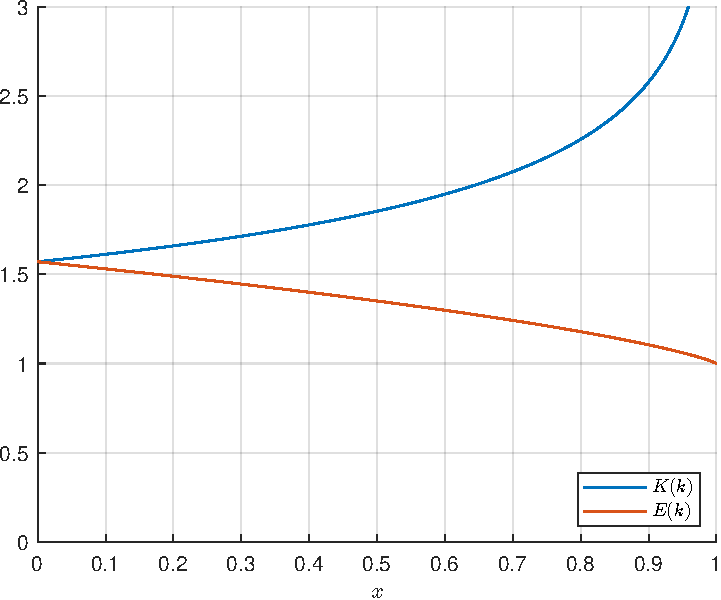
\includegraphics[width=7cm]{graphs/ellipseKE.pdf}
        \captionof{figure}{第一、二类完全椭圆积分}
    \end{center}
    当$r\gg a$或$r\ll a$或$\theta\to 0$时,
    \[
        A_\phi(r,\theta)=\frac{\mu_0I}4\frac{a^2r\sin\theta}{(a^2+r^2)^{3/2}}\biggfkh{1+\frac{15}8\biggkh{\frac{ar\sin\theta}{a^2+r^2}}^2+\cdots},
    \]
    因此对于$r\gg a$处的远场
    \begin{align*}
        B_r&=\frac1{r\sin\theta}\pp\theta(\sin\theta A_\phi)=\frac{\mu_0Ia^2}2\frac{\cos\theta}{r^3},\\
        B_\theta&=-\frac1r\pp r(rA_\theta)=\frac{\mu_0Ia^2}4\frac{\sin\theta}{r^3},
    \end{align*}
    与电偶极矩的电场\eqref{eqn:edipole-E}比较,可定义环形电流的磁偶极矩(magnetic dipole moment)大小
    \[
        m=I\cdot\pi a^2,
    \]
    沿$+z$方向,从而 
    \begin{align}
        \bm A&=\frac{\mu_0m\sin\theta}{4\pi r^2}\uvec\phi;\\
        \bm B&=\frac{\mu_0m}{4\pi r^3}(2\cos\theta\uvec r+\sin\theta\uvec\theta).
    \end{align}
\end{example}
我们现在考虑一般的电流分布在一个小(相对于感兴趣区域的尺度)的空间区域中的性质。
\footnote{这个问题可以用矢量球谐函数来做一个完整的处理,类似于静电多极展开。这些将在\chapref{chap:multipole radiation}多极辐射中介绍,我们在这里只满足于最低的近似阶。}
若$x\gg x'$,矢量势的分量可以被展开为:
\begin{equation}
    \label{eqn:A approx}
    A_\alpha(\bm x)=\frac{\mu_0}{4\pi}\biggfkh{\frac1{|\bm x|}\cancel{\int_V J_\alpha(\bm x')\d v'}+\frac{\bm x}{|\bm x|^3}\cdot\int_V J_\alpha(\bm x')\bm x'\d v+\cdots}
    \tag{$\ast$}
\end{equation}
下面我们用一些数学上的小tricks:
\[
    \oint_{\p V}fg\bm J\cdot\uvec n'\d a'=\int_V(g\bm J\cdot\nabla'f+f\bm J\cdot\nabla'g+fg\cancel{\nabla'\cdot\bm J})\d v'=0.
\]
将$f,g$赋予特定的形式,可以得到
\begin{alignat*}{2}
    \int_V J_\alpha \d v'&=0,&\qquad (f=1,\enspace g=x_\alpha');\\
    \int_V(x_\alpha'J_\beta+x_\beta'J_\alpha)\d v'&=0,&(f=x_\alpha',\enspace g=x_\beta')\\
    \int_V x_\alpha'J_\alpha\d v'&=0,&(f=g=x_\alpha').
\end{alignat*}
\begin{definition}{全反对称张量}{Levi-Civita symbol}
    引入全反对称张量(Levi-Civita symbol)
    \begin{equation}
        \epsilon_{\alpha\beta\gamma}=\begin{cases}
            1,&(\alpha\beta\gamma)=(123)\\
            -1,&(\alpha\beta\gamma)=(321)\\
            0,&\text{otherwise}
        \end{cases}
    \end{equation}
    一般地定义:$\epsilon_{1\cdots n}=1$,置换任意两个下标则反号,下标相同则为0。
\end{definition}
利用全反对称张量,我们可以将叉乘的结果记作
\begin{equation}
    (\bm a\times\bm b)_\alpha=\sum_{\beta,\gamma}\epsilon_{\alpha\beta\gamma}a_\beta b_\gamma.
\end{equation}
由此可得\eqref{eqn:A approx}中的积分项
\[
    \bm x'\cdot\int_V\bm x'J_\alpha\d v'=-\frac12\biggfkh{\bm x\times\int_V(\bm x'\times\bm J)\d v'}_\alpha.
\]
可定义磁矩密度(magnetic moment density)或磁化强度(magnetization)
\begin{equation}
    \bm M:=\frac12\bm x\times\bm J.
\end{equation}
其体积分为磁偶极矩(magnetic dipole moment)简称磁矩
\begin{equation}
    \bm m=\frac12\int_V\bm x'\times\bm J(\bm x')\d v'.
\end{equation}
因此式\eqref{eqn:A approx}中,矢量势的最低阶非零项
\begin{equation}
    \bm A(\bm x)=\frac{\mu_0}{4\pi}\frac{\bm m\times\bm x}{|\bm x|^3}.
\end{equation}
进而磁感应强度与电偶极矩电场\eqref{eqn:edipole-E with delta}形式相似:
\begin{equation}
    \bm B(\bm x)=\frac{\mu_0}{4\pi}\biggfkh{\frac{3\uvec n(\bm m\cdot\uvec n)-\bm m}{|\bm x|^3}+\frac{8\pi}3\bm m\vd(\bm x)}.
\end{equation}
因此,远离任何局域电流分布的磁场就是一个磁偶极子的磁场。
\begin{example}{电流回路的磁矩}{m of I}
    平面$S$上的电流回路的磁矩
    \begin{align*}
        \bm m=\frac12\oint_{\p S}\bm x\times I\d\bm\ell=IS\uvec n.
    \end{align*}
    与\exmref{exm:B of loop current} 中的定义一致。
\end{example}
\begin{example}{带电粒子轨道角动量的磁矩}{m of L}
    带电粒子的磁矩与其轨道角动量$\bm L=m\bm x\times\bm v$有关:
    \[
        \bm m=\frac12q\bm x\times\bm v=\frac q{2m}\bm L.
    \]
\end{example}
局部电流分布的磁场体积分
\[
    \int_{r<R}\bm B(\bm x)\d v=\begin{cases}
        \frac{2\mu_0}3\bm m,&\text{球内电流}\\[1ex]
        \frac{4\pi}3R^3\bm B(\bm 0),&\text{球外电流}
    \end{cases}.
\]

\subsection{磁矩的力、力矩和能量}
\label{ssec:force, torque and energy of magnetic moment}

外部磁感应强度$\bm B(\bm x)$中电流密度$\bm J(\bm x)$受到的总力
\[
    \bm F=\int_V\bm J(\bm x)\times\bm B(\bm x)\d v\simeq(\bm m\times\nabla)\times\bm B.
\]
化简为
\[
    \bm F=\nabla(\bm m\cdot\bm B)-\bm m\cancel{(\div\bm B)}.
\]
力矩与作用在磁偶极子上的力矩表达式相同:
\[
    \bm N=\int_V\bm x'\times(\bm J\times\bm B)\d v'\simeq\bm m\times\bm B(\bm 0),
\]
上式也可作为定义磁感应强度的一种方法。

由$\bm F=-\nabla U$,可定义磁矩的势能为
\[
    U=-\bm m\times\bm B,
\]
$U$并不是外磁场中磁矩的总能量,因为它不包含产生$\bm m$并维持$\bm m$恒定所需的能量。另外,当$\bm m$和$\bm B$方向相同时,$U$最低,因此磁矩倾向于偏转自己平行于磁场。

\section{宏观介质静磁学}
\label{sec:macroscopic magnetostatics}

在物质中,由原子电子贡献的有效(effective)原子电流和本征(intrinsic)磁矩产生的偶极场在原子尺度上变化非常明显。因此在宏观观测时,我们也需要对微观取空间平均\footnote{不需要对时间平均。}:
\begin{equation}
    \label{eqn:divB-macro}
    \div\bm B_\text{micro}=0\implies\div\bm B=0.
\end{equation}
在$\bm x'$由一个小体积的$\D V$产生的矢量势
\[
    \D\bm A(\bm x)\simeq\frac{\mu_0}{4\pi}\biggfkh{\frac{\bm J(\bm x)'}{|\bm x-\bm x'|}+\frac{\bm M(\bm x')\times(\bm x-\bm x')}{|\bm x-\bm x'|^3}}\D V.
\]
其中宏观磁矩密度
\[
    \bm M(\bm x):=\sum_iN_i\ave{\bm m_i},
\]
积分之
\[
    \bm A(\bm x)=\frac{\mu_0}{4\pi}\int_V\frac{\bm J(\bm x')+\nabla'\times\bm M(\bm x')}{|\bm x-\bm x'|}\d v'
\]
因此 
\[
    \curl\bm B=\mu_0(\bm J+\curl\bm M),
\]
其中$\bm J_\text M:=\curl\bm M$是有效电流密度。
定义磁场强度(magnetic field)
\begin{equation}
    \bm H:=\frac{\bm B}{\mu_0}-\bm M.
\end{equation}
从而 
\begin{equation}
    \label{eqn:curlH}
    \curl\bm H=\bm J.
\end{equation}
式\eqref{eqn:divB-macro}和\eqref{eqn:curlH}考虑了有效原子电流的贡献,是\eqref{eqn:divB}和\eqref{eqn:curlB}的宏观对应。
\paragraph{本构关系}
下面我们介绍$\bm H$和$\bm B$的本构关系。对于各向同性抗磁性(diamagnetic)和顺磁性(paramagnetic)物质,有简单的线性关系:
\[
    \bm B=\mu\bm H,
\]
$\mu$为磁导率(permeability)。对于顺磁性物质,$\mu\gtrapprox\mu_0$;抗磁性物质$\mu\lessapprox\mu_0$。铁磁性(ferromagnetic)物质的$\mu$与$\bm H$的关系较为复杂,存在磁滞现象(hysteresis),但由于其$\mu\gg\mu_0$,有时可对边界条件作出简化假设。
\paragraph{表面分布}
考虑介质界面上$\bm B$和$\bm H$的分布,我们可以得到:
\begin{align}
    \label{eqn:Bn2-Bn1}
    (\bm B_2-\bm B_1)\cdot\uvec n_{21}&=0,\\
    \label{eqn:Ht2-Ht1}
    (\bm H_2-\bm H_1)\times\uvec n_{21}&=\bm J_\text S,
\end{align}
当$\mu_1\gg\mu_2$时,$H_{2\text n}\gg H_{1\text n}$,磁场$\bm H_2$与边界面垂直。所以,极高磁导率材料表面上$\bm H$的边界条件与导体表面上$\bm E$的边界条件相同:
\begin{center}
	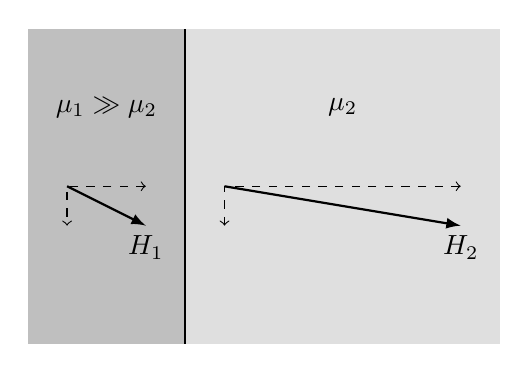
\begin{tikzpicture}
		\fill[gray!25](0, 0)rectangle(4, 4);
		\fill[gray!50](0, 0)rectangle(-2, 4);
		\node at(-1, 3){$\mu_1\gg\mu_2$};
		\node at(2, 3){$\mu_2$};
		\draw[thick](0, 0)--(0, 4);
		\draw[dashed, <->](-.5, 2)--(-1.5, 2)--(-1.5, 1.5);
		\draw[thick, -latex](-1.5, 2)--(-.5, 1.5)node[below]{$\bm H_1$};
		\draw[dashed, <->](3.5, 2)--(.5, 2)--(.5, 1.5);
		\draw[thick, -latex](.5, 2)--(3.5, 1.5)node[below]{$\bm H_2$};
	\end{tikzpicture}
	\captionof{figure}{极高磁导率材料表面的$\bm H$表现}
\end{center}
因此,我们可以把静电势理论用于磁场上,高磁导率材料的表面是近似的等势面。这种类比在许多磁铁设计问题中用到:先决定场的形式,然后把极面设计成等势面的形状。
\begin{example}{}{}
    对于真空中的极高磁导率材料,若其表面无电流,则
    \[
        H_\parallel=H_{0,\parallel},\quad B_\perp=B_{0,\perp},
    \]
    因此材料内磁场
    \[
        B^2=B_{0,\perp}^2+\frac{\mu^2}{\mu_0^2}B_{0,\parallel}^2.
    \]
    两边同除$\mu$便得到了能量密度的形式,由于材料中储存的能量是有限的,故$B_{0,\parallel}=0$
\end{example}

\subsection{静磁学中的边界条件问题}
\label{ssec:boundary-value problems in magnetostatics}

%对于磁化材料外部的磁场问题,
若材料是磁导率$\mu\gg\mu_0$的硬铁磁体(其磁矩密度$\bm M$与外场无关),则材料外表面上的$\bm B$垂直于界面,内表面上的$\bm B$平行于界面。如果其内没有电流($\bm J=\bm0$),则可引入磁势$\Phi_\text M$并解其Laplace方程。
\begin{equation}
    \bm H=-\nabla\bm\Phi_\text M,\quad\lapla\Phi_\text M=-\rho_\text M=\div\bm M.
\end{equation}
若无边界条件,则有解
\[
    \Phi_\text M=-\frac1{4\pi}\int_V\frac{\nabla'\cdot\bm M(\bm x')}{|\bm x-\bm x'|}\d v',
\]
若$\bm M$是局域的,则在$x\gg x'$的地方
\[
    \Phi_\text M\simeq\frac{\bm m\cdot\bm x}{4\pi r^3},\quad\bm m=\int_V\bm M\d v.
\]
但是我们仍需面对有边界条件的情形,在边界$\p V$处$\bm M$瞬间变为0,运用静电学中的结论:
\begin{equation}
    \label{eqn:PhiM with boundary}
    \Phi_\text M=-\frac1{4\pi}\int_V\frac{\nabla'\cdot\bm M(\bm x')}{|\bm x-\bm x'|}\d v'+\frac1{4\pi}\oint_{\p V}\frac{\bm M(\bm x')\cdot\uvec n'}{|\bm x-\bm x'|}\d a',
\end{equation}
若铁磁体是均匀磁化的,则$\div\bm M=0$,第一项为0。

我们接着求矢量势,由于$\bm J=\bm 0$,仅剩有效电流密度项
\begin{equation}
    \lapla\bm A=-\mu_0(\bm 0+\curl\bm M),
\end{equation}
可得
\begin{equation}
    \label{eqn:A with boundary}
    \bm A=\frac1{4\pi}\int_V\frac{\nabla'\times\bm M(\bm x')}{|\bm x-\bm x'|}\d v'+\frac1{4\pi}\oint_{\p V}\frac{\bm M(\bm x')\times\uvec n'}{|\bm x-\bm x'|}\d a',
\end{equation}
上式两项分别代表有效电流密度$\bm J_\text M$和有效面电流密度$\bm J_\text S$的贡献
\begin{align}
    \bm J_\text M&=\curl\bm M;\\
    \bm J_\text S&=\bm M\times\uvec n.
\end{align}
\begin{example}{均匀磁化球}{uniform magnetized sphere}
    真空中半径为$a$的球,其具有均匀的永久磁化强度$\bm M=M_0\uvec z$。应用式\eqref{eqn:PhiM with boundary}
    \[
        \Phi_\text M(r,\theta)=0+\frac1{4\pi}\oint_{r'=a}\frac{M_0\cos\theta'}{|\bm x-\bm x'|}\cdot a^2\d\Omega',
    \]
    进行球谐函数展开,式\eqref{eqn:1/|x-x'|=YY}仅有$\ell=1,\enspace m=0$项保留,且
    \[
        \cos\theta'=\sqrt{\frac{4\pi}3}Y_{10}(\theta',\phi'),
    \]
    故
    \[
        \Phi_\text M(r,\theta)=\frac13M_0a^2\cdot\frac{r_<}{r_>}\cos\theta.
    \]
    %$r_<,r_>$是$r,a$中的较小/大者。

    球内,$r_<=r,\enspace r_>=a$,表现为匀强磁场:
    \[
        \Phi_\text M=\frac13M_0r\cos\theta,\quad \bm H_\text{in}=-\frac13\bm M,\enspace\bm B_\text{in}=\frac{2\mu_0}3\bm M;
    \]
    球外,$r_<=a,\enspace r_>=r$,表现为磁偶极子(没有更高阶的项):
    \[
        \Phi_\text M=\frac{M_0a^3}3\frac{\cos\theta}{r^2}=\frac{\bm m\cdot\bm x}{4\pi r^3},\quad\bm m=\frac{4\pi}3a^3\bm M.
    \]
    $\bm B$线是连续的闭合曲线,而$\bm H$线不是。
    \tcblower
    也可通过矢量势的方法:
    \[
        A_\phi(r,\theta)=\frac{\mu_0}3M_0a^2\cdot\frac{r_<}{r_>^2}\sin\theta.
    \]
\end{example}
\begin{example}{外场下的磁化球}{magnetized sphere in external field}
    续\exmref{exm:uniform magnetized sphere},在全空间叠加一匀强场$\bm B_0=\mu_0\bm H_0$,便成为外场下的磁化球问题,球内场强为
    \[
        \bm H_\text{in}=\bm B_0+\frac{2\mu_0}3\bm M,\quad\bm H_\text{in}=\bm H_0-\frac13\bm M,
    \]
    如果球是顺磁或抗磁的,那么$\bm M$便是由外场引起的,且$\bm B_\text{in}=\mu\bm H_\text{in}$,从而得到与电介质\eqref{eqn:P-E}很相似的结果:
    \begin{equation}
        \label{eqn:M-B}
        \bm M=\frac3{\mu_0}\biggkh{\frac{\mu_\r-1}{\mu_\r+2}}\bm B_0.
    \end{equation}
    如果球是铁磁的,那么便可以得到$\bm B_\text{in}$和$\bm H_\text{in}$的限制关系:
    \[
        \bm B_\text{in}+2\mu_0\bm H_\text{in}=3\bm B_0,
    \]
    上式可以在磁滞图上画一条直线,并会产生交点。
\end{example}
\begin{example}{外场下的磁化球壳}{magnetized sphere shell in external field}
    内外半径为$a,b$的球壳磁导率为$\mu$,放置在匀强磁场$\bm B_0$中,由于没有电流可应用磁势求解
    \[
        \lapla\Phi_\text M=0
    \]
    由式\eqref{eqn:Phi(r, theta)},再加上$r\to\infty$时$\bm H=\bm H_0$的条件,可写出磁势的形式解,再通过边界条件
    \[
        \cdots
    \]
    \iffalse
    \begin{align*}
        \begin{cases}
            \edg{\pv{\Phi_\text{M,I}}\theta}_{r=a}=\edg{\pv{\Phi_\text{M,II}}\theta}_{r=a}\\[2ex]
            \edg{\pv{\Phi_\text{M,II}}\theta}_{r=b}=\edg{\pv{\Phi_\text{M,III}}\theta}_{r=b}
        \end{cases}
        \begin{cases}
            \mu_0\edg{\pv{\Phi_\text{M,I}}r}_{r=a}=\mu\edg{\pv{\Phi_\text{M,II}}r}_{r=a}\\[2ex]
            \mu_0\edg{\pv{\Phi_\text{M,II}}r}_{r=b}=\mu\edg{\pv{\Phi_\text{M,III}}r}_{r=b}
        \end{cases}
    \end{align*}
    \fi
    可得系数仅剩$\ell=1$项,壳内是一个匀强场:
    \[
        \Phi_\text M(r,\theta)=
        \begin{cases}
            a_1r\cos\theta,&r<a\\
            \ldots,&a<r<b\\
            -H_0r\cos\theta+\frac{d_1}{r^2}\cos\theta,&r>b
        \end{cases}
    \]
    当$\mu\gg\mu_0$时,壳内场强趋于0,这便是磁屏蔽效应。
\end{example}
最后探究了在一侧具有渐近均匀切向磁场的完全导电平面上的圆孔的影响,略。

\section{Faraday电磁感应定律}
\label{sec:Faraday}

我们在前几章里论述了静电学和静磁学中的稳恒态问题。我们虽然用了相似的数学方法,但把电现象和磁现象当作相互独立的现象来处理。两者之间唯一的联系在于如下事实:\textit{磁场是由电流产生的,而电流就是运动的电荷。}
但当我们考虑与时间有关的问题时,电现象和磁现象的几乎独立的性质便会消失:随时间变化的磁场会产生电场,反之亦然。%这时我们必须说电磁场,而不能说电场或磁场.只有在狭

Faraday在探究时变磁场中电流表现的实验表明:
\begin{compactenum}
    \item 接通/断开临近电路的稳恒电流;
    \item 临近电路的稳恒电流相对于本电路移动;
    \item 将一根永磁体插入/抽出电路
\end{compactenum}
都会在电路中产生瞬态(transient)电流。Faraday把瞬态电流的产生解释为电路环绕磁通量(magnetic flux)%\footnote{本笔记中,$\Phi$已经被标量势占用了,$\phi$被方位角占用了,$\psi$和$\varphi$似乎还没人占用。}
\begin{equation}
    \varPhi:=\int_S\bm B\cdot\uvec n\d a
\end{equation}
的变化所引起的。变化的磁通量会再电路周围感感生(induce)一个电场驱动电路电荷运动形成电流,其电动势(electromotive force, emf)为
\begin{equation}
    \emf:=\oint_{\p S}\bm E'\cdot\d\bm \ell.
\end{equation}
$\bm E'$是在运动坐标系或介质中的电场。则Faraday的观测结果可总结为:
\begin{equation}
    \label{eqn:emf propto varPhi'}
    \emf\propto-\dv\varPhi t.
    \tag{$\ast$}
\end{equation}
其符号由Lenz定律决定:感生电流磁通量总是对抗磁通量的变化。

\paragraph{Galileo变换}

下面我们希望得到式\eqref{eqn:emf propto varPhi'}中的比例系数$k$,%事实上此系数已经可以从已有的单位制推出,而不像$\varepsilon_0$等需要引入新的单位。
我们将从已有单位制推导(而非定义)该比例系数。

在狭义相对论(special relativity)发现之前(或处理低速情况时),所有物理学家都公认(虽然不经常明确说出)物理定律在Galileo变换(Galilean transformation):
\begin{align*}
    (t,\bm x)&\mapsto(t,\bm x+\bm vt),
\end{align*}
下应该是不变的。$\bm v$是两个参考系之间的相对速度。也就是说,两个以恒定速度$\bm v$作相对运动的观察者看到的物理现象是一样的。%,只要这两组空间坐标和时间坐标的关系遵从Galileo变换:

Faraday从实验上证实电磁感应现象在Galileo变换下不变:无论是载电流的初级电路静止、次级电路运动;或者是次级电路静止、而载电流的初级电路作同样的相对运动,在次级电路中感生的电流是相同的。

现在讨论一个运动电路的法拉第定律,如果电路以恒定速度$\bm v$移动,则磁场的迁移导数为
\begin{align*}
    \dv{\bm B}t&=\pv{\bm B}t+(\bm v\cdot\nabla)\bm B\\
    &=\pv{\bm B}t+\curl(\bm B\times\bm v)+\cancel{(\bm B\cdot\nabla)\bm v}-\bm B(\cancel{\div\bm v})+\bm v(\cancel{\div\bm B}),
\end{align*}
即,
\begin{align*}
    \dd t\int_S\bm B\cdot\uvec n\d a=\int_S\pv{\bm B}t\cdot\uvec n\d a+\oint_{\p S}(\bm B\times\bm v)\cdot\d\bm\ell,
\end{align*}
因此 
\[
    \oint_{\p V}\bigkh{\bm E'-k\bm v\times\bm B}\d\bm\ell=-k\int_S\pv{\bm B}t\cdot\uvec n\d a.
\]
由Galileo变换下电场力和Lorentz力的形式,应有:
\[
    \bm E'=\bm E+\bm v\times\bm B,
\]
即$k=1$,因此Faraday定律可以写成等式:
\begin{equation}
    \label{eqn:Faraday}
    \emf=-\dv\varPhi t,
\end{equation}
并可由Stokes公式转化为微分形式
\begin{equation}
    \label{eqn:curlE-B}
    \curl\bm E=-\pv{\bm B}t.
\end{equation}
而%我们知道
静电场的旋度\eqref{eqn:curlE}为0!由此可见,时变场将电场和磁场联系了起来。

\section{磁场的能量}
\label{sec:energy in the magnetic field}

我们在前面讨论静磁场时,避开了场能和能量密度的问题。
因为
要建立电流的稳恒组态及有关的磁场,必定经过一段初始的瞬变期,在这期间,电流和磁场从零增到终值。存在这种随时间变化的场,就存在使电流源做功的感生电动势。因为按照定义,场的能量等于建立这场时所做的总功,所以我们必须考虑这些贡献。

保持电流恒定不变,
\[
    \vd W=\int_V\vd\bm A\cdot\bm J\d v=\int_V\bm H\cdot\vd\bm B\d v.
\]
对于顺磁性和抗磁性物质,$2\bm H\cdot\vd\bm B=\vd(\bm H\cdot\bm B)$
\[
    W=\frac12\int_V\bm A\cdot\bm J\d v=\frac12\int_V\bm H\cdot\bm B\d v.
\]

将一个磁导率为$\mu$的物体放进电流源固定不动的磁场$\bm B$中,前后能量发生变化
\[
    \D W=\frac12\int_V\bm M\cdot\bm B_0\d v.
\]

\subsectionstar{自感和互感}
\label{ssec:self- and mutual inductance}

对于$N$个不导磁的载流电路系统,总能量可以描述为:
\[
    W=\frac12\sum_{i=1}^NL_iI_i^2+\frac12\sum_{i\neq j}M_{ij}I_iI_j.
\]
$L_i$是线圈$i$的自感(self-inductance),$M_{ij}$是线圈$i,j$之间的互感(mutual inductance),可以证明 
\[
    M_{ij}=M_{ji}.
\]

自感和互感可由
\[
    W=\frac12\int_V\bm J\cdot\bm A\d v.
\]
求出,用磁通量的形式即
\[
    L_i=\frac{\varPhi_{ii}}{I_i},\quad M_{ij}=\frac{\varPhi_{ij}}{I_j}.
\]
若电路是导磁的,则$W$的表达式不适用了,需要换为
\[
    W=\frac12\int_V\bm H\cdot\bm B\d v.
\]
后面还讨论了圆导线的自电感。

\sectionstar{似稳场}
\label{sec:quasi-static field}

似稳场(quasi-static field)、涡流(eddy current)、磁扩散(magnetic diffusion)

